% First draft — benchmark + geometric characterization paper
% \note{} marks placeholders that need content, numbers, or citations
\documentclass[review,onefignum,onetabnum]{./SIAM_template/siamart171218}
\usepackage[utf8]{inputenc}
\usepackage[T1]{fontenc}
\usepackage{amsmath}
\usepackage{amssymb}
\usepackage{amsfonts}
\usepackage{graphicx}
\usepackage{xcolor}
\usepackage{float}
\usepackage{hyperref}
\usepackage{booktabs}
\usepackage{url}
\usepackage[section]{placeins}
\usepackage[backend=bibtex]{biblatex}
\addbibresource{methods.bib}
\providecolor{RED}{rgb}{1,0,0}

\headers{STEROID: Inverse Buckingham Pi Dimensional Reduction}{V.\ Pustovoit et al.}

\newsiamremark{remark}{Remark}

% ---------------------------------------------------------------
% Note environment for first-draft placeholders
\newcommand{\note}[1]{\textcolor{red}{\textbf{[#1]}}}
% ---------------------------------------------------------------

\author{Vasilii Pustovoit \and Utkarsh Mali \and \note{co-authors?}}

%\title{Geometric Characterization of Feasible Parameter Spaces\\
%  in Buckingham Pi Dimensional Reduction:\\
%  Algorithm, Benchmark, and Extensions}
\title{Dimensional reduction on STEROIDs: Geometric Characterization of Feasible 
Parameter Spaces in Buckingham Pi}

\begin{document}
\maketitle

% ---------------------------------------------------------------
\begin{abstract}
We study the inverse dimensional reduction problem arising in Buckingham Pi analysis:
given a sampled point $\mathbf{d}$ in dimensionless space $\mathbb{R}^m$ and a map
$f$ encoding the Buckingham Pi exponents (linear: $A\mathbf{p}=\mathbf{d}$, or
non-linear monotonic), recover a physical parameter vector $\mathbf{p} \in \mathbb{R}^n$
satisfying the map and the physical constraints $\Lambda\mathbf{p} \leq \mathbf{c}$.
We present STEROID (Simplicial TEssellation Reduction Of Invariant Domains), which
preprocesses the feasible polytope once and answers subsequent queries in $O(1)$ time.
We benchmark STEROID against six alternative methods across a grid of problem sizes
$(n, m)$.  For \emph{point queries alone}, compiled Dykstra is faster
at $m \geq 4$ with zero preprocessing, with a crossover at $m \approx 3$--$4$:
the two methods scale in opposite directions with $m$, and no preprocessing
amortization justifies STEROID for pure feasibility queries.  
However, STEROID provides precomputed smooth $\partial\mathbf{p}/\partial\mathbf{d}$,
exact one-pass uniform sampling of the feasible dimensionless region,
non-linear monotonic extensions, and geometric characterization of the feasible
dimensionless region with no per-query analogue.
%We identify ultrasonic micro-injection molding process design as a concrete application
%where all three capabilities are simultaneously required: the inverse design map from
%target material properties to process parameters, its sensitivity surface
%$\partial E / \partial (A, U_t, P, T_M)$ for tolerance analysis, and exact feasibility
%characterization of the achievable operating region.
\end{abstract}

% ---------------------------------------------------------------
\section{Introduction}
\label{sec:intro}

Buckingham's $\Pi$-theorem \cite{Buckingham1914} states that any
physically meaningful equation involving $n$ dimensional quantities can be expressed in
terms of $m = n - k$ independent dimensionless groups, where $k$ is the rank of the
dimensional matrix (i.e. number of dimensions in kernel of the problem).
Dimensional analysis has become a core tool in fluid mechanics,
astrophysics, materials science, and engineering design~\cite{Bakarji2022,
BuckinghamPy2021, SalazarMeza2023, Opdahl2021}: working in dimensionless space
reduces experimental parameter sweeps from $n$-dimensional to $m$-dimensional.

\textbf{The inverse problem.}
Applications increasingly require the \emph{inverse} direction: given a query point
$\mathbf{d}$ sampled in dimensionless space (e.g., a grid point in a design sweep),
find one or more physical parameter vectors $\mathbf{p}$ that reproduce
$\mathbf{d}$ under the Buckingham map and satisfy all physical constraints
(ranges of validity, material limits, operating bounds).
This problem is under-determined---the preimage $A^{-1}\mathbf{d}$ is an affine
subspace of dimension $n - m$---and the constraint set restricts it to a (possibly
empty) convex polytope within that affine subspace.

To our knowledge, no dedicated open-source solver exists for this problem.
Gorard et al. \cite{Gorard2025} identify the lack of guarantees that
dimensionally reduced parameter combinations remain physically valid as an open
challenge in nuclear fusion and high-energy astrophysics.
Practitioners typically either resort to brute-force rejection sampling (prohibitively
slow), or run a linear program (LP) per query without exploiting the repeated
structure of the parameter sweep~\cite{Bakarji2022, BuckinghamPy2021}.

\textbf{Related work.}
In this paper we benchmark existing methods for solving the inverse dimensional
reduction problem and introduce a novel approach, STEROID, as an alternative.
The closest algorithmic relative is explicit linear Model Predictive Control
(MPC) \cite{Bemporad2002}, which precomputes a piecewise-affine (PWA) map from
parameter to optimizer by partitioning the parameter space into critical
regions via Karush-Kuhn-Tucker (KKT) conditions.  The resulting lookup table
supports $O(\log R)$ query cost ($R$ = number of regions) via binary search
trees \cite{Tondel2003}. The Delaunay Triangulation approach (a big part of
STEROID method) was also explored for explicit MPC by \cite{Scibilia2009}.

For feasibility queries without preprocessing, Dykstra's alternating projection
algorithm \cite{Dykstra1983, Tibshirani2017} solves the reduced LP formulation in the
null space of $A$ by cyclic projection onto half-spaces.  The HiGHS
solver \cite{HiGHS2022} provides a state-of-the-art LP simplex and interior-point
implementation.  Analytic centers of parameterized polytopes provide smooth selections via the
log-barrier function~\cite{Nesterov1998}, but require solving a convex
optimization problem at each query point.

%\textbf{When to use STEROID vs.\ alternatives.}
%A practitioner who needs only a \emph{single feasible point} per query should use
%Dykstra (C++): it requires no preprocessing and is faster at $m \geq 4$.
%STEROID's preprocessing overhead is only justified when the application requires
%one or more of the following:
%\begin{enumerate}
%  \item \emph{Smooth sensitivity}: $\partial\mathbf{p}/\partial\mathbf{d}$ as a
%    continuous function over the full feasible region (e.g., tolerance analysis,
%    gradient-based design optimization).  Per-query methods produce isolated points
%    with no mesh structure; derivatives cannot be formed.
%  \item \emph{Exact uniform sampling}: drawing unbiased samples from the feasible
%    physical parameter space (e.g., Monte Carlo UQ, training data generation).
%    LP/Dykstra cannot sample; MCMC is approximate.
%  \item \emph{Non-linear monotonic $f$}: when the dimensional reduction map is
%    coordinate-monotonic but not log-linear (e.g., Arrhenius kinetics, nonlinear
%    joint dynamics).  LP/Dykstra require convex feasibility; STEROID operates on
%    the physical polytope directly and is unaffected by non-linearity in $f$.
%  \item \emph{Very large query batches} ($Q \gtrsim 10^5$) with $m \leq 3$:
%    the $O(1)$ per-query cost amortizes preprocessing over many queries.
%\end{enumerate}
%
%\textbf{Contributions.}
%\begin{enumerate}
%  \item First systematic benchmark of methods for inverse Buckingham Pi dimensional
%    reduction, across an $(n,m)$ grid, with both Python and compiled C++ implementations.
%  \item Identification of opposite scaling laws: STEROID's per-query cost grows with
%    $m$ while Dykstra's shrinks, with crossover at $m \approx 3$--$4$.
%  \item Characterization of three capabilities unique to STEROID (smooth sensitivity,
%    exact sampling, non-linear monotonic $f$) that per-query methods cannot replicate.
%  \item Extension of STEROID to non-linear monotonic $f$ with approximation error
%    bounds from FEM interpolation theory.
%  \item A concrete worked application: ultrasonic micro-injection molding, where the
%    A matrix is read directly from published dimensional analysis, all constraints are
%    log-linear, and the inverse design + sensitivity problem is unsolved in the literature.
%  \item Theoretical analysis of GPU-friendly point location (spatial hashing, BVH)
%    that would eliminate the CGAL walk bottleneck and restore STEROID's per-query
%    advantage; empirical validation is deferred to future work.
%\end{enumerate}

The paper is organized as follows.
Section \ref{sec:problem} formalizes the inverse problem.
Section \ref{sec:nullspace} derives the null-space reduction exploited by all methods.
Section \ref{sec:methods} describes each method, including the full STEROID derivation
and correctness proof.
Sections \ref{sec:geometric}--\ref{sec:gpu} characterize STEROID's unique geometric
capabilities, non-linear extension, and GPU-friendly point location.
Section \ref{sec:experiments} describes the experimental setup,
Section \ref{sec:results} presents benchmark results,
Section \ref{sec:applications} demonstrates applications, and
Section \ref{sec:discussion} provides a method selection guide and discusses limitations.

% ---------------------------------------------------------------
\section{Problem Statement}
\label{sec:problem}

We work entirely in log-space.  Physical variables $\mathbf{p} \in \mathbb{R}^n$
are the logs of positive dimensional quantities; dimensionless variables
$\mathbf{d} \in \mathbb{R}^m$ are the logs of Buckingham groups; all constraints
are linear in these log variables.

\subsection{Physical space and constraints}

The physical parameter space is $\mathbb{R}^n$.  Physical constraints take the form
\begin{equation}
  \label{eq:constraint}
  \Lambda \mathbf{p} \leq \mathbf{c},
\end{equation}
where $\Lambda \in \mathbb{R}^{K \times n}$ and $\mathbf{c} \in \mathbb{R}^K$.
We assume the feasible set $\mathcal{P} = \{\mathbf{p} : \Lambda\mathbf{p} \leq
\mathbf{c}\}$ is a compact convex polytope (i.e., full-dimensional and bounded).

\subsection{Buckingham Pi map and dimensionless space}

By the Buckingham $\Pi$-theorem, there exists a matrix $A \in \mathbb{R}^{m \times n}$
with $\mathrm{rank}(A) = m < n$ such that the dimensionless variables are
\begin{equation}
  \label{eq:buckingham}
  A\mathbf{p} = \mathbf{d}.
\end{equation}
The feasible dimensionless region is $\mathcal{D}^* = \{A\mathbf{p} :
\mathbf{p} \in \mathcal{P}\}$, the projection of $\mathcal{P}$ under $A$.
This is itself a compact convex polytope in $\mathbb{R}^m$.

\subsection{Inverse problem}

Given a query $\mathbf{d} \in \mathbb{R}^m$, find $\mathbf{p} \in \mathbb{R}^n$
satisfying \eqref{eq:constraint} and \eqref{eq:buckingham}, or report infeasibility.
Return $\emptyset$ if $\mathbf{d} \notin \mathcal{D}^*$.

In practice, queries arrive as a batch $G = \{\mathbf{d}_1, \ldots, \mathbf{d}_Q\}$
(e.g., a regular $11^m$-point Cartesian grid in $[-1,1]^m$), and the problem
parameters $A, \Lambda, \mathbf{c}$ are fixed across all queries.

% ---------------------------------------------------------------
\section{Null-Space Reduction}
\label{sec:nullspace}

All methods in this paper exploit the following algebraic reduction.

\begin{proposition}
  \label{prop:nullspace}
  The general solution to $A\mathbf{p} = \mathbf{d}$ is
  \begin{equation}
    \label{eq:nullspace}
    \mathbf{p} = A^\dagger \mathbf{d} + N\mathbf{z}, \qquad \mathbf{z} \in \mathbb{R}^{n-m},
  \end{equation}
  where $A^\dagger \in \mathbb{R}^{n \times m}$ is the Moore-Penrose pseudoinverse and
  $N \in \mathbb{R}^{n \times (n-m)}$ is a basis for $\ker(A)$.  Substituting into
  \eqref{eq:constraint} reduces the problem to an LP in $\mathbb{R}^{n-m}$:
  \begin{equation}
    \label{eq:reduced_lp}
    (\Lambda N)\mathbf{z} \leq \mathbf{c} - \Lambda A^\dagger \mathbf{d}.
  \end{equation}
\end{proposition}

The key observation is that \eqref{eq:reduced_lp} lives in $\mathbb{R}^{n-m}$, not
$\mathbb{R}^n$.  As $m$ increases (holding $n$ fixed), the LP dimension $n - m$
\emph{decreases}.  Any per-query method exploits this automatically.

% ---------------------------------------------------------------
\section{Methods}
\label{sec:methods}

\subsection{LP Simplex and Interior Point (HiGHS)}
\label{sec:lp}

The most direct approach: solve \eqref{eq:reduced_lp} as an LP feasibility problem
with HiGHS \cite{HiGHS2022}.  Simplex is exponential in the worst case but
typically performs $O((n{-}m) K)$ pivot steps in practice;
interior point achieves polynomial worst-case $O((n{-}m)^{3.5} \log(1/\varepsilon))$.
No preprocessing beyond computing $N$, $A^\dagger$ once ($O(n^2 m)$ via SVD).

\subsection{Chebyshev Center LP}
\label{sec:chebyshev}

Find the Chebyshev center of \eqref{eq:reduced_lp}: the largest inscribed ball
maximizes minimum slack, giving the most ``interior'' feasible point.
Solved as an LP with one additional radius variable~\cite{Boyd2004}.
Useful when downstream applications require $\mathbf{p}$ to be far from
constraint boundaries.

\subsection{Dykstra's Alternating Projection}
\label{sec:dykstra}

Dykstra's algorithm \cite{Dykstra1983} finds the projection onto the intersection of
convex sets by cyclic orthogonal projection with incremental corrections.
Applied to \eqref{eq:reduced_lp}: project $\mathbf{z}$ onto each half-space
$(\Lambda N)_k \mathbf{z} \leq (\mathbf{c} - \Lambda A^\dagger \mathbf{d})_k$
in round-robin order.  Projection onto one half-space costs $O(n-m)$.
Per-query scaling is then $O(C \cdot K \cdot (n-m))$, $C \approx 5$--$20$
cycles in practice, which decreases as $m$ increases.

Dykstra terminates when the maximum constraint violation falls below a
tolerance $\varepsilon$.  The returned point satisfies
$(\Lambda N)_k \mathbf{z} \leq (\mathbf{c} - \Lambda A^\dagger \mathbf{d})_k
+ \varepsilon$ for all $k$, so feasibility holds up to $\varepsilon$.

\subsection{ADMM and Kaczmarz}
\label{sec:admm_kaczmarz}

Alternating Direction Method of Multipliers (ADMM) \cite{BoydADMM2011} solves 
the feasibility problem via consensus splitting,
with similar per-iteration cost to Dykstra but easier parameter tuning for
ill-conditioned constraint matrices.  ADMM converges in $O(1/\varepsilon)$
iterations for the feasibility residual.
Randomized Kaczmarz \cite{Strohmer2009} uses random constraint selection and
converges exponentially in expectation:
$\mathbb{E}\|\mathbf{z}_t - \mathbf{z}^*\|^2 \leq (1 - \kappa^{-2})^t
\|\mathbf{z}_0 - \mathbf{z}^*\|^2$, where $\kappa$ is the scaled condition
number of $\Lambda N$.
A gradient-penalty method adds a differentiable penalty
$\rho \|\max(0,\, (\Lambda N)\mathbf{z} - (\mathbf{c} - \Lambda A^\dagger
\mathbf{d}))\|^2$ to a quadratic objective and minimizes via gradient descent,
increasing $\rho$ progressively until feasibility is achieved.

\subsection{STEROID: Vertex Enumeration + Delaunay Triangulation}
\label{sec:steroid}

STEROID invests in a one-time preprocessing step: it identifies the feasible
region, projects it into dimensionless space, triangulates it, and precomputes
an affine map for each simplex.  Subsequent queries reduce to locating
the containing simplex and evaluating a single matrix-vector product.

We now walk through the construction step by step.

\subsubsection{Identifying the feasible vertices}

The feasible polytope $\mathcal{P} = \{\mathbf{p} : \Lambda\mathbf{p} \leq
\mathbf{c}\}$ is defined by $K$ linear constraints (its H-representation).
STEROID first converts $\mathcal{P}$ to its V-representation---a list of vertices
$W = \{\mathbf{w}_1, \ldots, \mathbf{w}_V\}$---using the Parma Polyhedra
Library \cite{PPL2008}.  By McMullen's Upper Bound Theorem \cite{McMullen1970},
which bounds the number of faces of a polytope with $K$ facets in $\mathbb{R}^n$,
the vertex count satisfies $V \leq \binom{K}{\lfloor n/2 \rfloor}$.

\subsubsection{Projection into dimensionless space}
\label{sec:proj_dim_subspace}

Each vertex $\mathbf{w}_i \in \mathbb{R}^n$ is mapped to dimensionless space via
$\mathbf{v}_i = A\mathbf{w}_i \in \mathbb{R}^m$.  The projected vertices
$\{\mathbf{v}_1, \ldots, \mathbf{v}_V\}$ span the feasible dimensionless region
$\mathcal{D}^*$.

\textbf{Degenerate projections.}  Multiple physical vertices may project to the same
(or nearly the same) dimensionless point when the polytope $\mathcal{P}$ has edges
nearly aligned with $\ker(A)$.  In this case the Delaunay triangulation produces
near-degenerate simplices ($\det P_i \approx 0$), and the deprojection matrix
$E_i = P_i' P_i^{-1}$ becomes ill-conditioned.  A natural remedy, left for future implementation, is to merge projected
vertices within a relative tolerance $\varepsilon_{\mathrm{merge}}$ before
triangulation, retaining among merged candidates the parent vertex farthest
from all constraint boundaries (maximizing slack).

\subsubsection{Triangulating the dimensionless region}

We compute the Delaunay triangulation of the projected vertices using
CGAL \cite{cgal}, producing a set of simplices $\{T_1, \ldots, T_S\}$ that
partition $\mathcal{D}^*$.  In the worst case,
$S = O(V^{\lceil m/2 \rceil})$ \cite{McMullen1970}.

\subsubsection{Obtaining physical values from a query point}

Now take an arbitrary simplex $T_i$ and a query point $\mathbf{d}$ inside it.
Each simplex has $m+1$ vertices in dimensionless space; we pick one as the
``base'' vertex $\mathbf{v}_{i,0}$ and form the difference vectors from it.
Any point $\mathbf{d}$ inside $T_i$ can then be written as:
\begin{equation}
  \label{eq:steroid_1}
  \mathbf{d} = \mathbf{v}_{i,0} + \sum_{j=1}^{m} \mu_j
    (\mathbf{v}_{i,j} - \mathbf{v}_{i,0}).
\end{equation}
Where we solve for $\vec{\mu} = \left\{ \mu_i \right\}$.
If no simplex contains $\mathbf{d}$, then
$\mathbf{d} \notin \mathcal{D}^*$ and we report infeasibility.

To get the physical parameters, we remember that each projected vertex
$\mathbf{v}_{i,j}$ has a ``parent'' vertex $\mathbf{w}_{i,j}$ in physical space
(the vertex that was projected to produce it: $A\mathbf{w}_{i,j} = \mathbf{v}_{i,j}$).
We apply the \emph{same} barycentric coordinates $\mu_j$ to the parent vertices:
\begin{equation}
  \label{eq:steroid_2}
  \mathbf{p} = \mathbf{w}_{i,0} + \sum_{j=1}^{m} \mu_j
    (\mathbf{w}_{i,j} - \mathbf{w}_{i,0}).
\end{equation}

\subsubsection{Precomputing the deprojection map}

Since the difference vectors in \eqref{eq:steroid_1} and \eqref{eq:steroid_2}
depend only on the simplex (not on the query point), we can precompute
everything into a compact form.

Define $P_i \in \mathbb{R}^{m \times m}$ as the matrix whose columns are the
difference vectors $\mathbf{v}_{i,j} - \mathbf{v}_{i,0}$ for $j=1,\ldots,m$,
and $P_i' \in \mathbb{R}^{n \times m}$ as the matrix whose columns are the
corresponding physical differences
$\mathbf{w}_{i,j} - \mathbf{w}_{i,0}$.

With this notation, \eqref{eq:steroid_1} becomes
$\mathbf{d} = \mathbf{v}_{i,0} + P_i \boldsymbol{\mu}$.
Since $T_i$ is a non-degenerate simplex, $\det P_i \neq 0$, and we can solve
for the barycentric coordinates:
\begin{equation}
  \label{eq:steroid_mu}
  \boldsymbol{\mu} = P_i^{-1}(\mathbf{d} - \mathbf{v}_{i,0}).
\end{equation}

Substituting into \eqref{eq:steroid_2}:
\begin{equation}
  \label{eq:steroid_expand}
  \mathbf{p} = \mathbf{w}_{i,0} + P_i' P_i^{-1}(\mathbf{d} - \mathbf{v}_{i,0})
  = \mathbf{w}_{i,0} - P_i' P_i^{-1}\mathbf{v}_{i,0} + P_i' P_i^{-1} \mathbf{d}.
\end{equation}

The first two terms give a vector that depends only on the simplex.  The last
term is a matrix (also depending only on the simplex) multiplied by the query
point.  We can therefore write:
\begin{equation}
  \label{eq:steroid_final}
  \mathbf{p} = \mathbf{e}_i + E_i\,\mathbf{d}, \qquad
  E_i = P_i' P_i^{-1}, \qquad
  \mathbf{e}_i = \mathbf{w}_{i,0} - E_i\,\mathbf{v}_{i,0}.
\end{equation}
Both $\mathbf{e}_i \in \mathbb{R}^n$ and $E_i \in \mathbb{R}^{n \times m}$ are
computed once per simplex during preprocessing and stored for retrieval.

\subsubsection{Query evaluation}

At query time, STEROID performs two operations:
\begin{enumerate}
  \item \emph{Point location}: find the simplex $T_i$ containing $\mathbf{d}$
    via CGAL's triangulation walk---starting from a previously located simplex
    and following facet adjacencies until $\mathbf{d}$ is enclosed.
  \item \emph{Affine map}: compute $\mathbf{p} = \mathbf{e}_i + E_i \mathbf{d}$
    (one matrix-vector multiply, $O(nm)$ operations).
\end{enumerate}
If the walk exits the convex hull of $\mathcal{D}^*$, the query is infeasible.
The deprojection data $(\mathbf{e}_i, E_i)$ can also be evaluated in batch:
a matrix of query points yields a matrix of physical parameters, making the
linear algebra embarrassingly parallel.

\subsubsection{Correctness}

The key property of this construction is that it always produces a feasible
physical point.

\begin{theorem}
  \label{thm:feasibility}
  For any $\mathbf{d}$ interior to a simplex $T_i \subset \mathcal{D}^*$, the
  deprojected point $\mathbf{p} = \mathbf{e}_i + E_i \mathbf{d}$ satisfies:
  (i)~$A\mathbf{p} = \mathbf{d}$, and
  (ii)~$\Lambda\mathbf{p} \leq \mathbf{c}$.
\end{theorem}
\begin{proof}
  Since $\mathbf{d}$ lies inside $T_i$, the barycentric coordinates
  $\mu_j \geq 0$ with $\sum_j \mu_j \leq 1$.  Setting
  $\mu_0 = 1 - \sum_{j=1}^m \mu_j$, the deprojected point is
  $\mathbf{p} = \sum_{j=0}^m \mu_j \mathbf{w}_{i,j}$---a convex combination
  of the physical vertices.
  Since $A\mathbf{w}_{i,j} = \mathbf{v}_{i,j}$ by construction:
  $A\mathbf{p} = \sum_j \mu_j \mathbf{v}_{i,j} = \mathbf{d}$.
  Since each $\mathbf{w}_{i,j} \in \mathcal{P}$ and $\mathcal{P}$ is convex,
  $\mathbf{p} \in \mathcal{P}$, i.e., $\Lambda\mathbf{p} \leq \mathbf{c}$.
\end{proof}

\begin{remark}
  The deprojection map $\mathbf{d} \mapsto \mathbf{p}$ is piecewise affine and
  generally \emph{discontinuous} across simplex boundaries: adjacent simplices
  $T_i$ and $T_j$ sharing a facet may have different parent vertices, producing
  different $\mathbf{p}$ values at the shared boundary.  Feasibility is preserved
  (both outputs lie in $\mathcal{P}$ and satisfy $A\mathbf{p} = \mathbf{d}$), but
  the map is multi-valued at boundaries.  The $C^k$ spline interpolation of
  Section \ref{sec:splines} resolves this by enforcing smoothness across simplex
  boundaries.
\end{remark}

\subsubsection{Scaling}

The per-query cost has two components:
(i)~the triangulation walk, costing $O(S^{1/m})$ simplex traversals in
expectation (each requiring $O(m)$ facet tests), giving $O(m \cdot S^{1/m})$;
and (ii)~the matrix multiply $E_i \mathbf{d}$, costing $O(nm)$.
Both grow with $m$, making STEROID \emph{slower} as $m$ increases---the
opposite scaling from Dykstra.

Preprocessing is dominated by the Delaunay triangulation, with worst-case
$O(V^{\lceil m/2 \rceil})$ simplices.  This becomes impractical for $m \geq 6$.

% ---------------------------------------------------------------
\section{Complexity Summary}
\label{sec:complexity}

\begin{table}[h]
\caption{Asymptotic complexity.  $K$: constraints; $n,m$: dimensions;
  $V \sim K^{\lfloor n/2 \rfloor}$: vertices; $C$: convergence cycles.
  $\dagger$Typical-case; simplex is exponential in the worst case.}
\label{tab:complexity}
\centering
\begin{tabular}{lllll}
\toprule
Method & Preprocessing & Per query & Memory & Trend in $m$ \\
\midrule
LP simplex   & $O(1)$ & $O((n{-}m) K)$\textsuperscript{$\dagger$} & $O(nK)$ & Gets faster \\
LP IPM       & $O(1)$ & $O((n{-}m)^{3.5})$ & $O(nK)$ & Gets faster \\
Chebyshev    & $O(1)$ & $O((n{-}m) K)$\textsuperscript{$\dagger$} & $O(nK)$ & Gets faster \\
Dykstra      & $O(1)$ & $O(C K(n{-}m))$ & $O(nK)$ & Gets faster \\
ADMM         & $O(1)$ & $O(C K(n{-}m))$ & $O(nK)$ & Gets faster \\
Kaczmarz     & $O(1)$ & $O(C(n{-}m))$ & $O(nK)$ & Gets faster \\
STEROID      & $O(V^{\lceil m/2 \rceil})$ & $O(m \cdot S^{1/m} + nm)$ & $O(V^{\lceil m/2\rceil} n)$ & Gets slower \\
\bottomrule
\end{tabular}
\end{table}

% ---------------------------------------------------------------
\section{Geometric Capabilities of STEROID}
\label{sec:geometric}

Beyond point queries, STEROID's triangulation enables tasks inaccessible to per-query
methods.

\subsection{Feasible volume computation}

\begin{equation}
  \mathrm{vol}(\mathcal{D}^*) = \sum_i \frac{|\det P_i|}{m!}.
\end{equation}
Exact, $O(S m^3)$ (one determinant per simplex).  Monte Carlo alternatives converge as $O(1/\sqrt{N})$.
Application: uncertainty quantification---``what fraction of dimensionless design
space is physically realizable?''

\subsection{Exact uniform sampling}

To sample uniformly in dimensionless space $\mathcal{D}^*$: select simplex $T_i$
with probability $\propto |\det P_i|/m!$ (proportional to its volume); sample
$\mathbf{d} \sim \mathrm{Uniform}(T_i)$ via Dirichlet$(1,\ldots,1)$ barycentric
coordinates; recover $\mathbf{p} = \mathbf{e}_i + E_i \mathbf{d}$.

To sample uniformly in \emph{physical} space $\mathcal{P}$, the simplex selection
probabilities must be adjusted by the Jacobian of the deprojection map: select $T_i$
with probability $\propto |\det P_i| \cdot |\det(E_i^\top E_i)|^{1/2} / m!$, which
accounts for the volume distortion of the affine map $E_i$ from $\mathbb{R}^m$ to
$\mathbb{R}^n$.  Both variants are exact one-pass samplers.  The Volesti
library~\cite{volesti} provides hit-and-run MCMC sampling within polytopes,
but requires a burn-in period of $O(n^3)$ steps before samples are
approximately uniform, and the approximation error is controlled only in
distribution.  STEROID's sampler produces exactly uniform samples with no
burn-in and no tolerance parameter.

\subsection{Phase diagrams of active constraint sets}

Each physical constraint $(\Lambda\mathbf{p})_k \leq c_k$ is either
\emph{active} (tight, $= c_k$) or \emph{inactive} (strict, $< c_k$) at a given
point $\mathbf{p}$.  The set of active constraints changes as $\mathbf{d}$ moves
through $\mathcal{D}^*$: in one region of dimensionless space the amplitude bound
may be the binding constraint, while in another it may be the temperature bound.
Knowing which constraint is active at each operating point is directly useful for
engineering: it tells the designer which physical limit is the bottleneck for each
target dimensionless state.

STEROID makes this information available without any additional computation.
For each simplex $T_i$, the parent vertices $\{\mathbf{w}_{i,0}, \ldots,
\mathbf{w}_{i,m}\}$ already lie on the boundary of $\mathcal{P}$, so their
active constraint sets $\mathcal{A}_{i,j} = \{k : (\Lambda\mathbf{w}_{i,j})_k
= c_k\}$ are known from the vertex enumeration step.  We define the dominant
active set of simplex $T_i$ as the union $\mathcal{A}_i = \bigcup_j
\mathcal{A}_{i,j}$.  Coloring each simplex in the triangulation by
$\mathcal{A}_i$ produces a map in $\mathcal{D}^*$ showing which physical
constraints govern each region of dimensionless space---a phase diagram in the
thermodynamic sense.

In explicit MPC~\cite{Tondel2003}, a similar map is produced via KKT critical
regions, where each region corresponds to exactly one active set by construction.
STEROID's Delaunay simplices are determined by geometry rather than optimality,
so a single simplex may nominally span two active sets near a transition; the
phase diagram is therefore an approximation near boundaries between phases,
improving as the triangulation is refined.

\subsection{Smooth $d \to p$ manifolds via spline interpolation}
\label{sec:splines}

The Delaunay triangulation provides a simplicial mesh on $\mathcal{D}^*$ suitable for
$C^k$ spline interpolation \cite{LaiSchumaker2007}.  Replacing the piecewise-affine
STEROID map with a $C^k$ spline yields:
\begin{itemize}
  \item Analytical sensitivity: $\partial\mathbf{p}/\partial\mathbf{d}$ available
    everywhere in $\mathcal{D}^*$.
  \item Smooth optimization on the feasible manifold.
  \item Geodesic computation with well-defined curvature.
\end{itemize}
The analytic center \cite{Nesterov1998} achieves $C^\infty$ but requires online
optimization per query.  STEROID + splines achieves $C^k$ with precomputed $O(1)$ evaluation.
Constructing splines that are continuous across simplex boundaries (i.e.,
achieving $k \geq 1$) requires choosing the spline coefficients to satisfy
inter-element compatibility conditions; this is a standard problem in finite
element analysis~\cite{LaiSchumaker2007, Ciarlet2002} and is deferred to
future work.

% ---------------------------------------------------------------
\section{Extension to Non-Linear Monotonic Maps}
\label{sec:nonlinear}

\begin{definition}
  $f: \mathbb{R}^n \to \mathbb{R}^m$ is \emph{coordinate-monotonic} if each $f_j$
  is monotonically increasing or decreasing in each $p_i$ separately.
\end{definition}

Physical examples include Arrhenius reaction rate laws
($k \propto e^{-E_a/RT}$, monotone in temperature $T$), Cobb-Douglas production
functions ($Y = A K^\alpha L^\beta$, monotone in capital $K$ and labor $L$), and
power-law rheology models where viscosity depends monotonically on shear rate
and temperature~\cite{SalazarMeza2023, RomeroObon2025}.

\begin{proposition}
  \label{prop:nonlinear}
  If $f$ is coordinate-monotonic and $\mathcal{P}$ is a compact convex polytope, then
  the vertices of $\mathcal{P}$ map to extreme points of $f(\mathcal{P})$.
\end{proposition}

Note that $f(\mathcal{P})$ is \emph{not} necessarily convex for general
coordinate-monotonic $f$.  However, the STEROID pipeline does not require convexity
of $f(\mathcal{P})$: it only requires that the Delaunay triangulation of the projected
vertices covers the region of interest.  In practice, we triangulate the convex hull
of $\{f(\mathbf{w}_i)\}$, which is a convex superset of $f(\mathcal{P})$.  Query points
that fall inside the convex hull but outside $f(\mathcal{P})$ will still receive a
deprojected $\mathbf{p}$ that satisfies $\mathbf{p} \in \mathrm{conv}(\mathcal{P})
= \mathcal{P}$ (by convexity of $\mathcal{P}$), but with $f(\mathbf{p}) \neq \mathbf{d}$
in general---the deprojected point is feasible but the forward map is only approximate.
For coordinate-monotonic $f$ that are additionally \emph{componentwise convex} (or
concave), $f(\mathcal{P})$ is itself convex and the convex hull equals $f(\mathcal{P})$
exactly.

The STEROID pipeline proceeds as before: enumerate vertices of $\mathcal{P}$, project
via $f$ (function evaluation rather than matrix multiply), triangulate.  The per-simplex
map becomes a piecewise-linear approximation to $f^{-1}$.

\textbf{Approximation error.}  Since $f$ is under-determined ($m < n$), $f^{-1}$ is
not a function in the classical sense.  However, STEROID's piecewise-linear
construction implicitly selects a \emph{section} $\sigma: \mathcal{D}^* \to
\mathcal{P}$ (a right inverse of $f$) defined by the barycentric interpolation
of parent vertices.  Let $\sigma^*$ denote the ``true'' section that would be
obtained by exact inversion (e.g., the section passing through the same parent
vertices with $f(\sigma^*(\mathbf{d})) = \mathbf{d}$ exactly).  On each simplex
$T_i$ with diameter $h_i$, $\sigma$ agrees with $\sigma^*$ at the vertices, so by
standard multivariate Lagrange interpolation error \cite{Ciarlet2002}:
\begin{equation}
  \label{eq:error_bound}
  \|\sigma(\mathbf{d}) - \sigma^*(\mathbf{d})\|
  = O\!\left(h_i^2 \|D^2 \sigma^*\|_\infty\right).
\end{equation}
Finer triangulation (more vertices or adaptive refinement) reduces $h_i$ and
improves accuracy, but also increases precompute time.

\textbf{Uniqueness.}  Explicit MPC requires $f = A$ (linear).  Analytic center and
Dykstra require convex $f(\mathcal{P})$ (non-linear $f$ may destroy convexity).
Differentiable convex optimization layers~\cite{cvxpylayers} embed a convex
program as a layer in a neural network, enabling gradient-based learning through
the solution map; but this still requires $f(\mathcal{P})$ to be convex at each
forward pass.  Only STEROID operates directly on $\mathcal{P}$, avoiding any
convexity requirement on $f$.

% ---------------------------------------------------------------
\section{GPU-Friendly Point Location (Projected Performance)}
\label{sec:gpu}

The current STEROID bottleneck for large batches is CGAL's triangulation walk
(pointer-chasing, cache-unfriendly on GPU).  The matrix multiply $E_i \mathbf{d}$
is already perfectly SIMD-parallel.

\subsection{Spatial hashing}

During preprocessing, insert each simplex into a hash table keyed by the Morton
code (Z-order curve)~\cite{MortonCode1966}
of its bounding grid cell.  Per-query: one hash lookup
$O(1)$ + $O(m)$ barycentric containment check.

\begin{table}[h]
\caption{Estimated per-query FLOPs with spatial-hash point location ($C=10$ for
  Dykstra).  \note{Verify with hardware benchmarks.}}
\label{tab:gpu_flops}
\centering
\begin{tabular}{rrrrr}
\toprule
$m$ & $n$ & STEROID (hash+matmul) & Dykstra & STEROID speedup \\
\midrule
2 &  6 & $\sim 12$  & $\sim 960$  & $\sim 80\times$ \\
3 &  6 & $\sim 18$  & $\sim 660$  & $\sim 37\times$ \\
5 &  6 & $\sim 30$  & $\sim 330$  & $\sim 11\times$ \\
5 & 10 & $\sim 50$  & $\sim 750$  & $\sim 15\times$ \\
8 & 12 & $\sim 96$  & $\sim 1080$ & $\sim 11\times$ \\
\bottomrule
\end{tabular}
\end{table}

\subsection{BVH for higher dimensions}

Morton encoding requires $>64$ bits for $m \geq 9$.  A Bounding Volume Hierarchy
(BVH) provides $O(m \log V)$ point location.  NVIDIA RTX cores include dedicated BVH
traversal hardware applicable to simplex point location.

\subsection{Warp-divergence advantage}

Dykstra's variable iteration count causes GPU warp divergence: threads in a
warp must wait for the slowest query before proceeding, wasting compute on
well-conditioned queries.  STEROID's fixed-cost pipeline (one lookup + one
matmul) eliminates warp divergence entirely, providing a fundamental
architectural advantage for large batches on GPU.  Empirical quantification
via CUDA profiling is deferred to future work.

% ---------------------------------------------------------------
\section{Experimental Setup}
\label{sec:experiments}

\subsection{Problem generation}

We generate synthetic problems on an $(n,m)$ grid with $n \in \{4,6,8,10,12,15,20\}$
and $m \in \{2,3,4,5,6,8\}$ (valid pairs: $m < n$).  For each pair:
\begin{enumerate}
  \item $A \in \mathbb{R}^{m \times n}$: random normal, orthogonalized to
    $\mathrm{rank}(A) = m$.
  \item $K = 3(n+m)$ constraints: $\Lambda \in \mathbb{R}^{K \times n}$ with entries
    in $[-1,1]$; $\mathbf{c}$ shifted to ensure feasibility.
  \item Query set $G$: $11^m$-point Cartesian grid in $[-1,1]^m$, capped at 500.
\end{enumerate}

\subsection{Implementation}

Python methods (LP simplex, LP IPM, Chebyshev) use HiGHS via the
\texttt{highspy} Python bindings with default solver settings.
Dykstra, ADMM, Kaczmarz, gradient penalty, and LP-HiGHS are implemented as
standalone C++ binaries compiled with \texttt{-O3 -march=native} and linked
against HiGHS~\cite{HiGHS2022}.
STEROID is compiled with the same flags, using CGAL~\cite{cgal} for
triangulation and PPL~\cite{PPL2008} for vertex enumeration.
For each method, preprocessing (matrix factorizations, triangulation) is timed
separately from per-query evaluation.  Python method timings reflect
interpreter overhead; C++ timings are hardware-limited.

\subsection{Timing}

Per method, we record: preprocessing time $t_{\mathrm{pre}}$ (s), mean per-query
time $t_{\mathrm{q}}$ (ms), $p_{99}$ query time, and feasibility rate.
$N_{\mathrm{rep}} = 5$ repetitions; median reported.
\textbf{Hardware:} \note{CPU model, RAM, OS, compiler version.}

% ---------------------------------------------------------------
\section{Results}
\label{sec:results}

\subsection{Per-query speed}

Figure \ref{fig:speed_heatmaps} shows mean query time across the $(n,m)$ grid.

\begin{figure}[h]
  \centering
  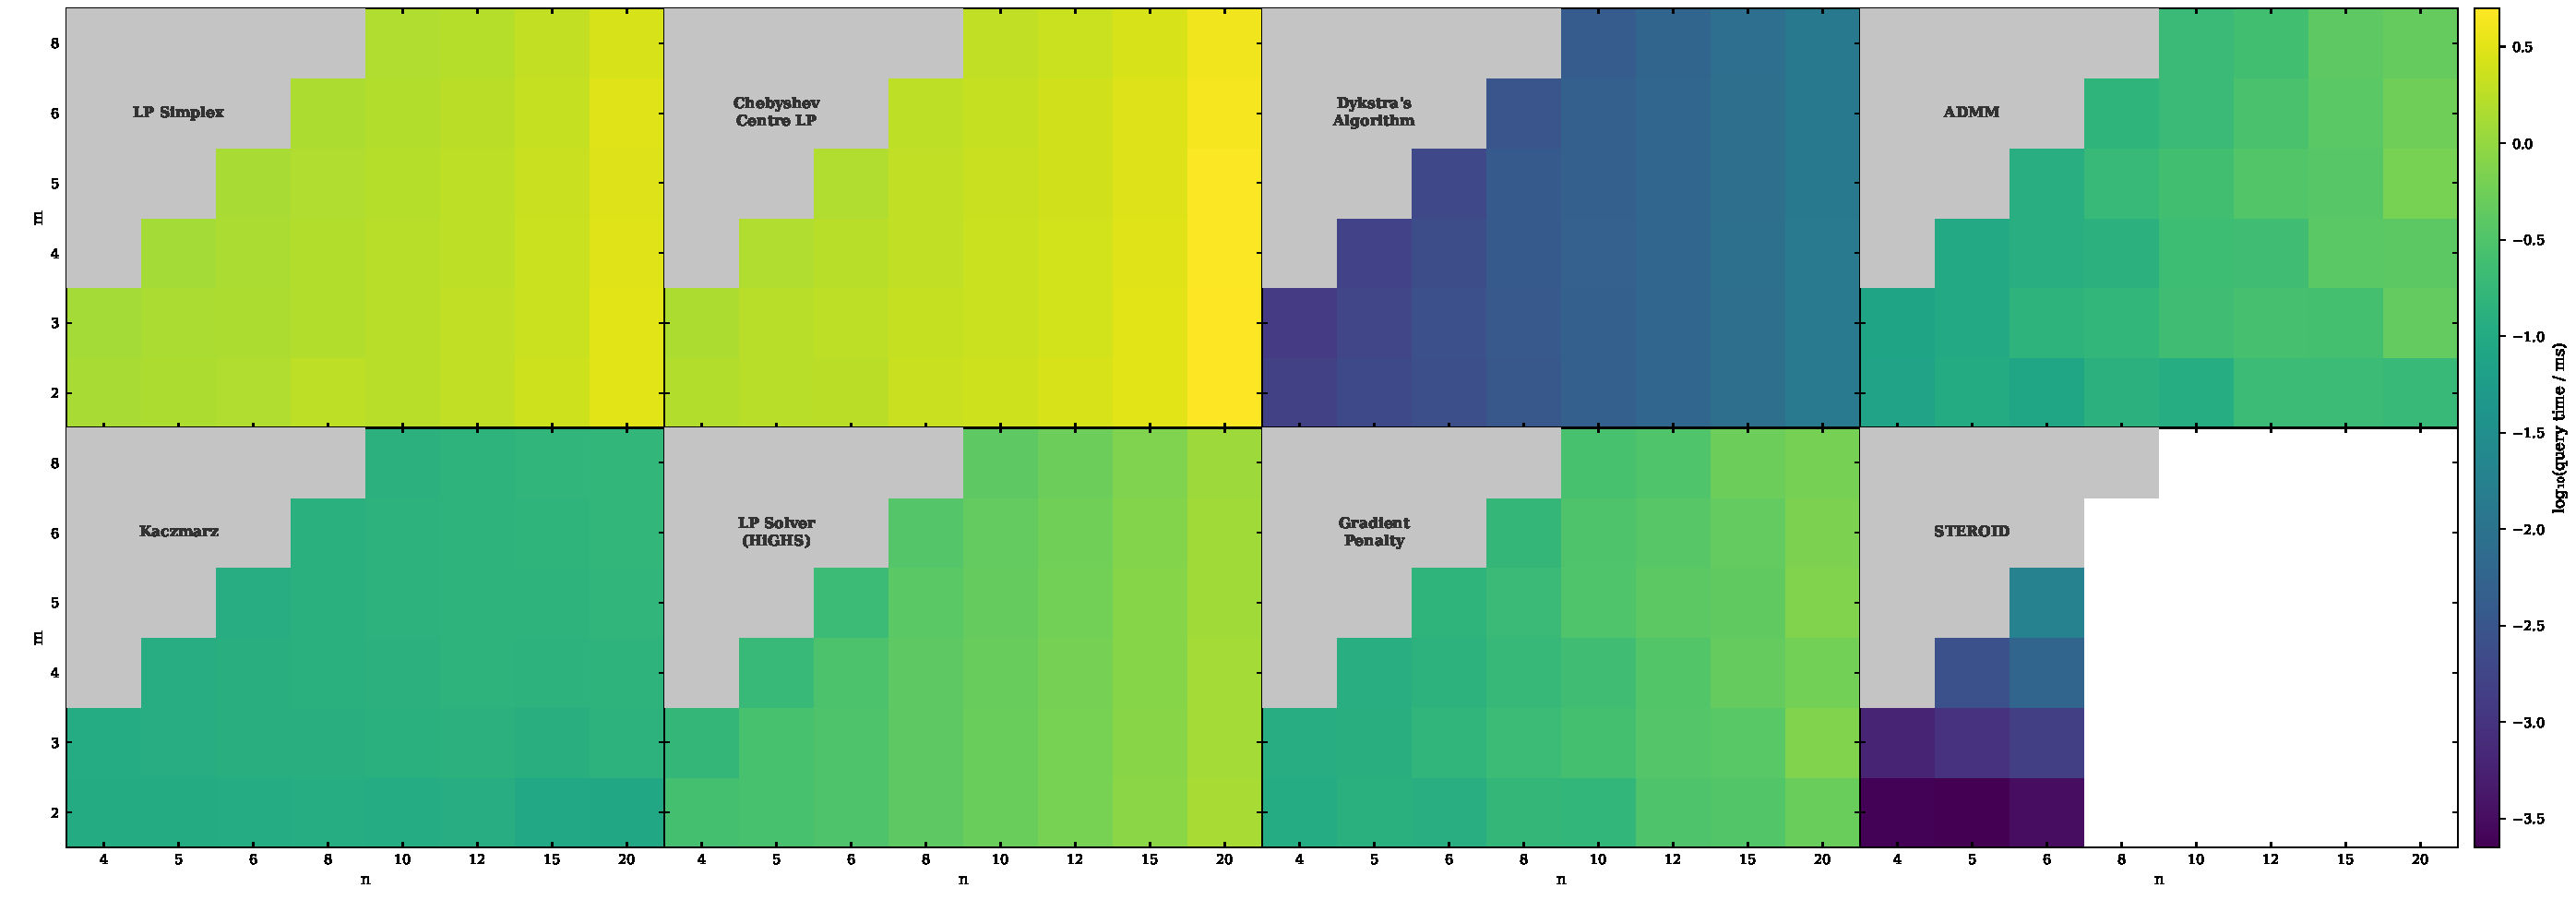
\includegraphics[width=\textwidth]{plots/speed_heatmaps.pdf}
  \caption{Mean query time (ms, log scale) vs.\ $(n,m)$ per method.
    White: missing data (timeout or infeasible preprocessing).}
  \label{fig:speed_heatmaps}
\end{figure}

C++ Dykstra achieves $0.001$--$0.013$~ms per query across all tested pairs with zero
preprocessing.  STEROID is ${\sim}7\times$ faster at $m=2$ and
${\sim}10\times$ slower at $m=5$.  Crossover at $m \approx 3$--$4$,
consistent with opposite scaling predicted in Section \ref{sec:methods}.
Python LP methods are ${\sim}100$--$3000\times$ slower than Dykstra; C++ LP-HiGHS
is ${\sim}30$--$100\times$ slower.

\subsection{Preprocessing}

Figure \ref{fig:preproc_heatmaps} shows preprocessing time.

\begin{figure}[h]
  \centering
  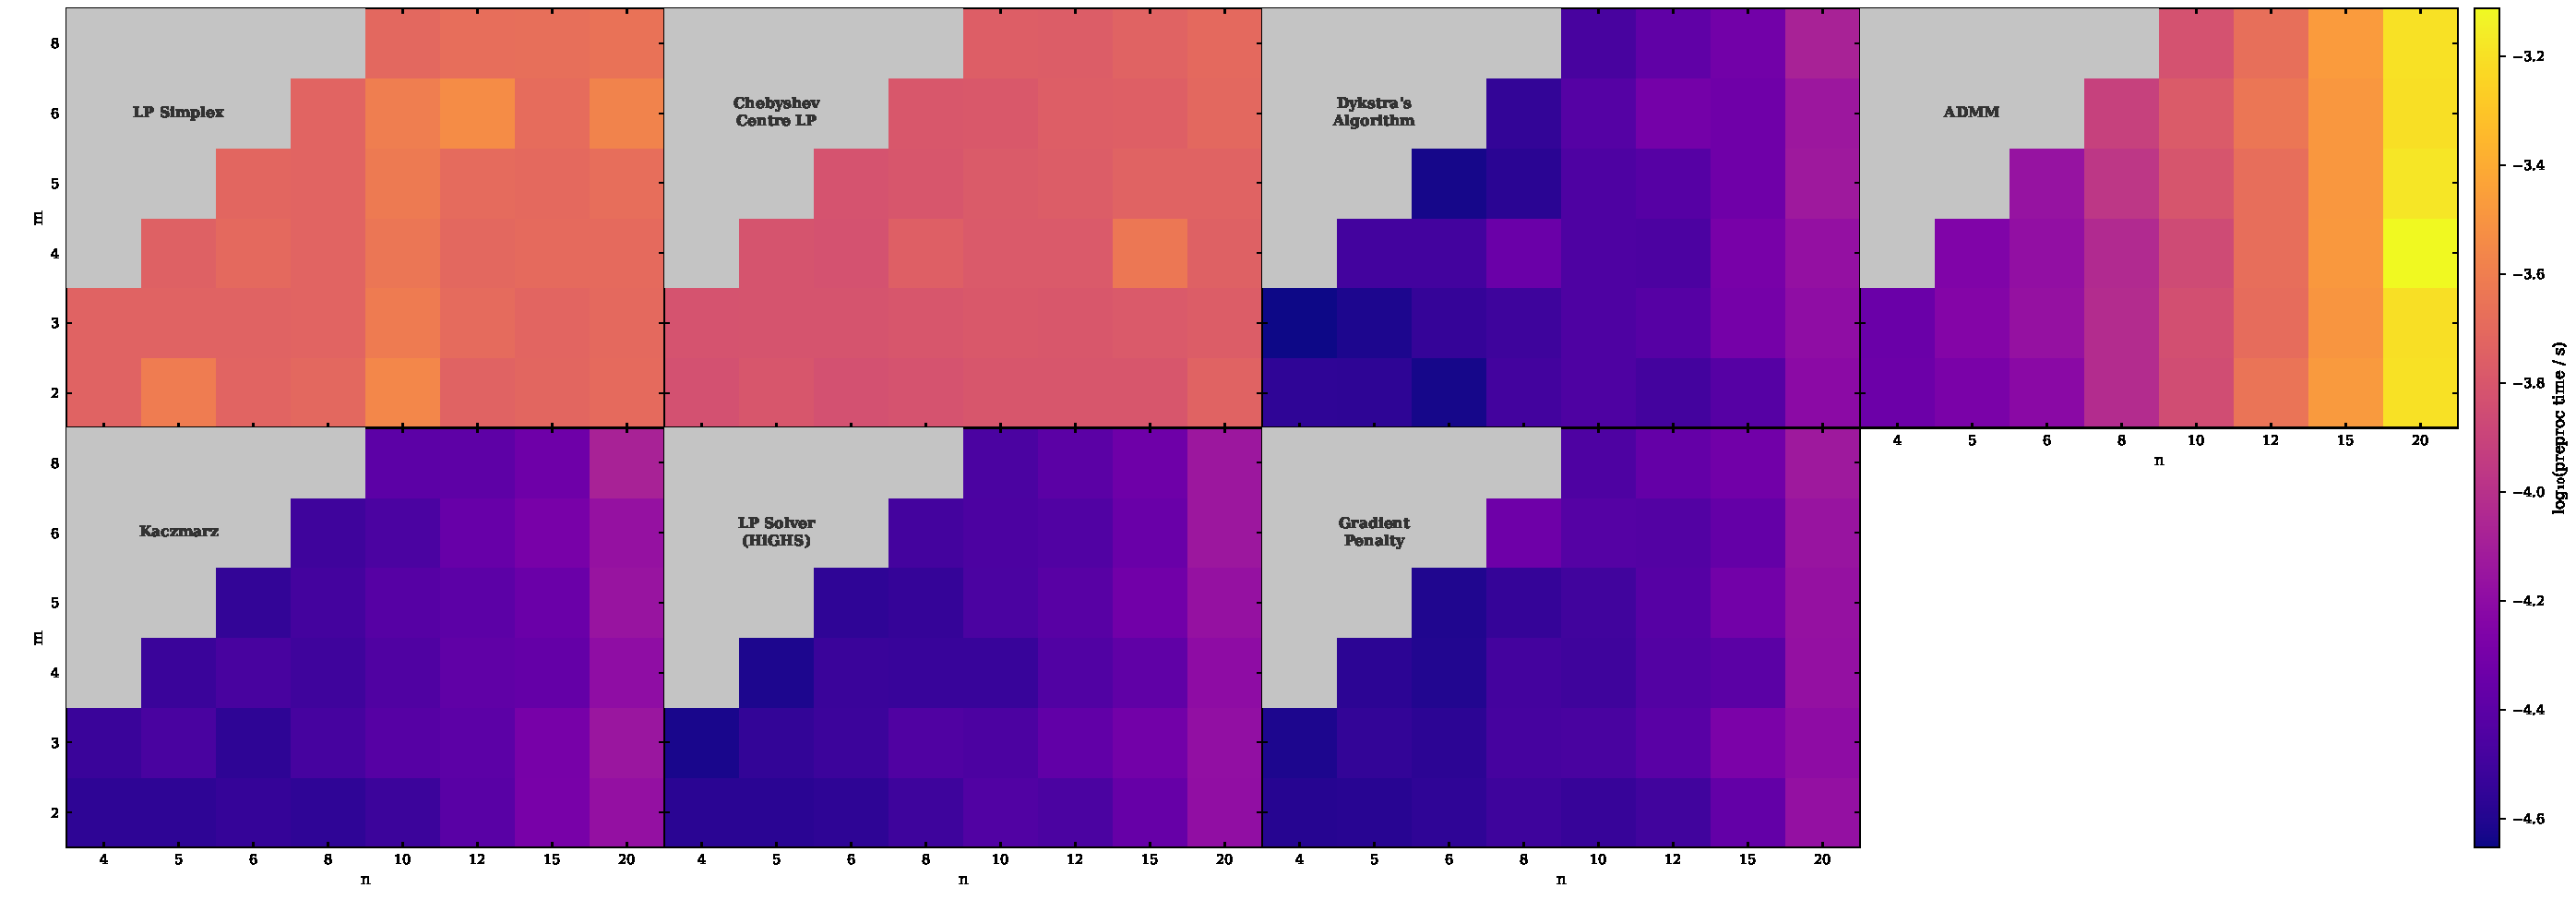
\includegraphics[width=\textwidth]{plots/preproc_heatmaps.pdf}
  \caption{Preprocessing time (s, log scale) vs.\ $(n,m)$.
    White: exceeded timeout or not tested.}
  \label{fig:preproc_heatmaps}
\end{figure}

STEROID preprocessing grows exponentially in $m$ and becomes infeasible at
$m \geq 6$ in our tests (the largest tested STEROID instance, $n=6$, $m=5$,
requires ${\sim}0.09$~s).
All per-query methods have $\leq 1$~ms preprocessing (SVD of $A$ only).

\subsection{Break-even query count}

Figure \ref{fig:breakeven} shows $Q^* = t_{\mathrm{pre}}^{\mathrm{STEROID}} /
(t_{\mathrm{q}}^{\mathrm{method}} - t_{\mathrm{q}}^{\mathrm{STEROID}})$
for $(n,m)$ pairs where STEROID is faster per query ($m \leq 3$).

\begin{figure}[h]
  \centering
  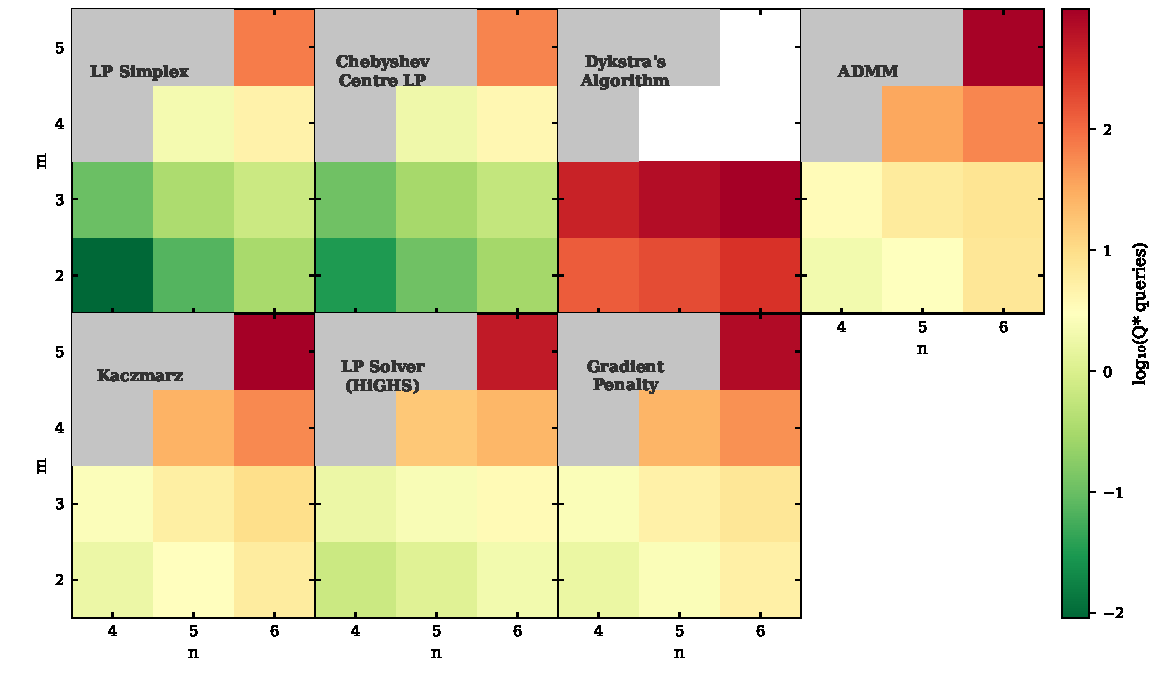
\includegraphics[width=\textwidth]{plots/breakeven_heatmap.pdf}
  \caption{Break-even query count $\log_{10}(Q^*)$ for $(n,m)$ pairs where
    STEROID has per-query advantage.  Red = many queries to amortize; blue = few.}
  \label{fig:breakeven}
\end{figure}

At $m=2$, STEROID preprocessing takes $0.0002$--$0.0008$~s (depending on $n$),
while the per-query advantage over Dykstra is ${\sim}0.002$~ms.  This gives
$Q^* \approx 100$--$400$ queries to break even---comparable to the standard $11^2 = 121$
grid.
At $m=3$, preprocessing takes $0.0003$--$0.0016$~s with a per-query advantage of
${\sim}0.001$~ms, giving $Q^* \approx 300$--$1600$.  The standard $11^3 = 1331$ grid
approaches break-even at the larger $(n,m)$ pairs.

\subsection{Speedup vs.\ STEROID}

Figure \ref{fig:speedup} shows per-query speedup of each method relative to STEROID.

\begin{figure}[h]
  \centering
  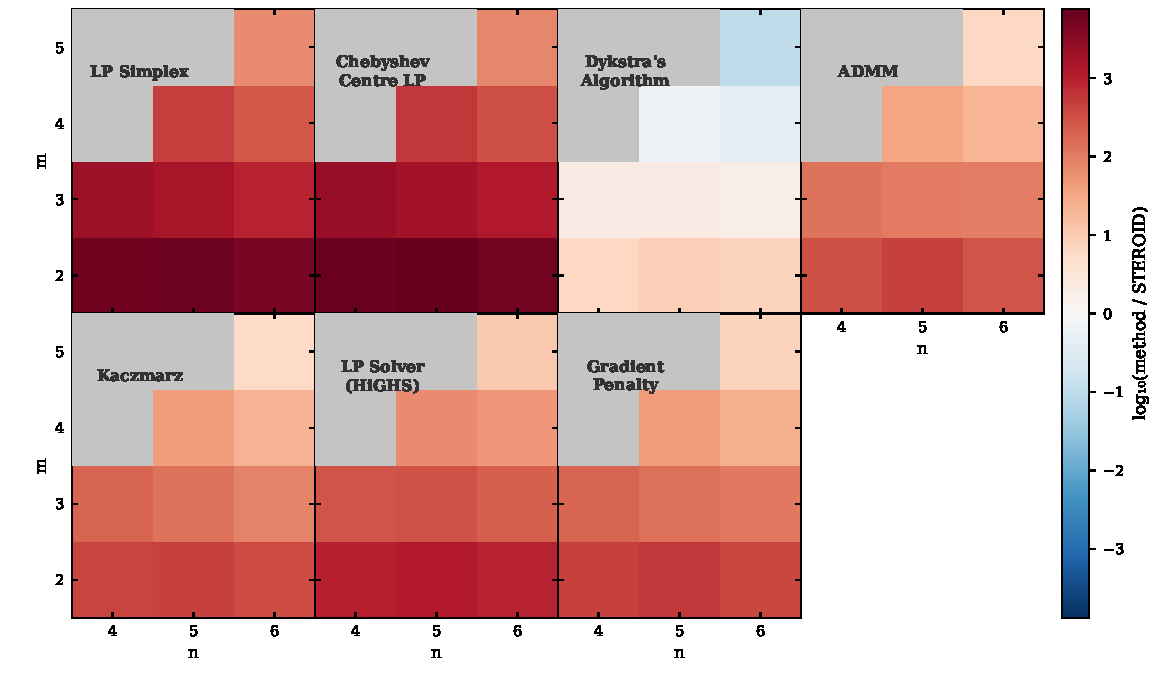
\includegraphics[width=\textwidth]{plots/speedup_heatmaps.pdf}
  \caption{Query speedup vs.\ STEROID (log ratio; blue = faster than STEROID).}
  \label{fig:speedup}
\end{figure}

Dykstra is faster than STEROID for all tested pairs with $m \geq 4$.

% ---------------------------------------------------------------
\section{Applications}
\label{sec:applications}

We now demonstrate STEROID's unique capabilities on two concrete applications drawn
from the literature, selected because they require capabilities that per-query methods
genuinely cannot provide.  We also discuss two motivating examples where STEROID
addresses an open gap identified in the literature, even though full numerical
demonstrations are deferred.

\subsection{Ultrasonic micro-injection molding: inverse design and sensitivity}
\label{sec:molding}

Salazar-Meza et al. \cite{SalazarMeza2023} apply Buckingham Pi analysis to ultrasonic
micro-injection molding (UMIM), fitting power-law models for energy consumption $Q$
and final Young's modulus $E$ of the molded part.  With $n=7$ physical variables
(amplitude $A$, action time $U_t$, plunger power $P$, flexural modulus $S_f$, mold
temperature $T_M$, thermal conductivity $\lambda$, output property) and $m=3$
dimensionless groups ($\Pi_0 = Q/(U_t P)$, $\Pi_1 = A^4 S_f T_M \lambda / (U_t P^2)$,
$\Pi_2 = A^3 E / (U_t P)$), the fitted models read in log-space:
\begin{align}
  \log E &= \log(5.82{\times}10^{-8}) - 1.03\log A + 0.508\log U_t
            + 0.016\log P + 0.492\log(S_f T_M \lambda), \notag \\
  \log Q &= \log(9.05{\times}10^{5}) + 2.20\log A + 0.449\log U_t
            - 0.101\log P + 0.551\log(S_f T_M \lambda). \notag
\end{align}
The exponent matrix $A$ is read directly from these equations.  Process constraints
are log-linear box bounds: $A \in [22.5, 56.2]\ \mu\text{m}$,
$U_t \in [4, 5]\ \text{s}$, $\text{IF} \leq 4000\ \text{N}$,
$T_M \in [323, 373]\ \text{K}$, plus the feasibility threshold
$\log\Pi_1 > -9\log 10$ (which is also linear in log-space).

\textbf{Gap in the existing work.}
The paper solves only the \emph{forward} direction---given process parameters, predict
$E$ and $Q$.  It explicitly leaves the inverse problem unsolved: given a target Young's
modulus $E^*$, which combinations of $(A, U_t, P, T_M)$ achieve it within the feasible
operating window?  The paper identifies infeasible combinations empirically by
discarding trials that fail to produce complete specimens.

\textbf{What STEROID provides.}
\begin{enumerate}
  \item \emph{Inverse design}: for any target $(E^*, Q^*)$, STEROID returns a
    feasible process parameter set in $O(1)$ after preprocessing.  The feasible
    region in $(\Pi_1, \Pi_2)$ space is a polytope image; its preimage covers all
    achievable operating points.
  \item \emph{Sensitivity surface}: via $C^k$ splines on the triangulation,
    $\partial E / \partial A$, $\partial E / \partial U_t$, etc.\ are available
    as continuous functions over the entire feasible operating space.  A process
    engineer can identify the most sensitive parameter direction and allocate
    manufacturing tolerance budgets accordingly.  No per-query method produces
    this: LP gives one point at a time with no mesh.
  \item \emph{Feasibility characterization}: STEROID computes the exact volume of the
    achievable $(\Pi_1, \Pi_2)$ region and identifies which constraint---amplitude
    bound, power bound, or temperature bound---is active at each operating point.
\end{enumerate}

\note{If time permits: implement the UMIM STEROID run numerically and show the
sensitivity surface plot as a figure here.}

\subsection{Dimensionless robot policy transfer: hardware feasibility}
\label{sec:robot}

Girard \cite{Girard2024} and Hromatko et al. \cite{Hromatko2025} show that control
policies trained in dimensionless space transfer zero-shot to any physically similar
system.  For a pendulum, the dimensionless context is $\mathbf{d} = (q^*, \tau^*_{\max})
= (q/(mgl),\ \tau_{\max}/(mgl))$; for a race car, $m=5$ dimensionless groups
encode mass ratios and scaled traction coefficients.  The Buckingham Pi maps are power-law monomials and hence linear in log-space
(Theorem~1 of \cite{Girard2024} establishes this for the pendulum; the race car
uses the same monomial structure but the log-linearity should be verified from the
specific group definitions in each application).

\textbf{Gap identified in the literature.}
Both papers prove that many physical systems map to the same $\mathbf{d}$, but neither
provides an algorithm for finding which hardware configurations are feasible:
``\emph{Equation~(12) is a mapping from a $m$ dimensional space to a $m{-}d$
dimensional space, and its inverse has multiple solutions}'' \cite{Girard2024}
(here $d$ denotes the number of base dimensions in the original text, not our
dimensionless vector $\mathbf{d}$).
Transferring a trained policy requires identifying real hardware (within actuator
datasheets and structural bounds) that achieves the target $\mathbf{d}$.

\textbf{What STEROID provides.}
The hardware constraint polytope (motor torque bounds, mass range, link length range
from a parts catalogue) is log-linear.  STEROID precomputes the image of this polytope
in $\mathbf{d}$-space---the set of dimensionless operating points achievable with
available hardware---and answers ``does hardware configuration $\mathbf{p}$ achieve
$\mathbf{d}^*$?'' in $O(1)$.  For the more practically important question of finding
the full family of hardware achieving $\mathbf{d}^*$, STEROID provides exact uniform
sampling and the phase diagram of binding constraints (e.g., torque limit vs.\ mass
limit vs.\ link length limit).

\textbf{Non-linear extension.}
Real robot joints have nonlinear inertia and friction terms.  If the forward map
$\mathbf{d} = f(\mathbf{p})$ is coordinate-monotonic but not log-linear (e.g.,
nonlinear joint stiffness), LP-per-query becomes non-convex and fails.
STEROID's non-linear monotonic extension is the only method that handles this case.

\subsection{Open gap: inverse dimensional reduction in fusion reactor design}
\label{sec:fusion}

Gorard et al. \cite{Gorard2025} identify the problem of ensuring physical
validity of dimensionally reduced parameter combinations as an open challenge
in nuclear fusion and astrophysics.  For tokamak design, the energy confinement scaling laws (IPB98,
DS03) are power laws in plasma temperature, density, magnetic field, and geometry,
and the Greenwald density limit, Troyon beta limit, and kink stability factor are
all log-linear constraints---the full STEROID problem structure.

We note, however, that replacing STEROID here requires care: the expensive step in
existing reactor dimensioning studies (e.g., \cite{Sarazin2019}) is a self-consistent
nonlinear system solve per design point, not an LP.  STEROID addresses the
\emph{linear sub-problem} (which parameter combinations satisfy the scaling law and
linear constraints), not the full nonlinear reactor code.  Its value would be in
providing precomputed sensitivity $\partial(R, B, \beta_N) / \partial(\text{exponents})$
for uncertainty propagation through the scaling law, and in generating unbiased
samples from the feasible reactor design space for Bayesian inference---neither of
which a per-query LP provides.

% ---------------------------------------------------------------
\section{Discussion}
\label{sec:discussion}

\subsection{When to use STEROID vs.\ Dykstra}

A critical finding of our benchmark is that STEROID's preprocessing overhead is
\emph{not} justified by per-query speed alone: Dykstra is faster at $m \geq 4$
with zero preprocessing.  STEROID is the right choice only when the application
genuinely requires one of its unique capabilities.

\begin{table}[h]
\caption{Method selection guide.  ``Point query'' = find any feasible $\mathbf{p}$
  for a given $\mathbf{d}$.}
\label{tab:selection}
\centering
\begin{tabular}{p{5.5cm}l}
\toprule
Need & Recommended method \\
\midrule
Point query only, $m \geq 4$                     & Dykstra (C++)       \\
Point query only, $m \leq 3$, $Q \gtrsim 10^5$  & STEROID             \\
Smooth $\partial\mathbf{p}/\partial\mathbf{d}$ everywhere & STEROID + splines \\
Exact uniform sampling                           & STEROID             \\
Non-linear monotonic $f$                         & Extended STEROID    \\
Feasible volume or phase diagram                 & STEROID             \\
$m \geq 6$, any task                             & Dykstra             \\
Certifiably exact solution                       & LP (HiGHS)          \\
\bottomrule
\end{tabular}
\end{table}

For pure point queries at $m \geq 4$, Dykstra requires no preprocessing and is
faster per query than STEROID; there is no benefit to the preprocessing cost.
At $m \leq 3$ with very many queries ($Q \gtrsim 10^5$), STEROID's $O(1)$
per-query cost can amortize the preprocessing over the batch.
When smooth sensitivity $\partial\mathbf{p}/\partial\mathbf{d}$ is required
over all of $\mathcal{D}^*$---for tolerance analysis or gradient-based
design optimization---LP and Dykstra are inapplicable: they return isolated
points with no mesh structure, and derivatives cannot be formed across queries.
Exact uniform sampling of the feasible space is similarly beyond LP or Dykstra;
Volesti's MCMC is an approximation with burn-in cost.
When the forward map $f$ is coordinate-monotonic but not log-linear, convexity
of the feasibility domain is not guaranteed and LP/Dykstra may fail;
STEROID operates on $\mathcal{P}$ directly and is unaffected.
At $m \geq 6$, STEROID's preprocessing grows exponentially and Dykstra becomes
the only practical option.
When a certifiably exact solution is required, LP via HiGHS~\cite{HiGHS2022}
is preferable to Dykstra (which has a finite termination tolerance); STEROID is
exact in the linear case by Theorem~\ref{thm:feasibility}.

\textbf{Common misconception.}
It is tempting to argue STEROID is justified whenever preprocessing can be paid once
and many queries follow.  This is true only at $m \leq 3$ (where STEROID is faster
per query) and $Q \gtrsim 10^5$.  For $m \geq 4$ and any realistic query count,
Dykstra is faster \emph{in total} (preprocessing + all queries).  The correct
justification for STEROID in those regimes is always one of the unique capabilities
in Table \ref{tab:selection}, not amortized query speed.

\subsection{Relationship to explicit MPC}
\label{sec:mpc_comparison}

STEROID computes the same mathematical object as explicit MPC \cite{Bemporad2002}:
a precomputed piecewise-affine lookup table that maps a low-dimensional parameter
$\mathbf{d}$ to a feasible solution $\mathbf{p}$.  The connection is genuine: both
partition a bounded parameter domain into regions and precompute an affine map per
region.  However, the two approaches differ in how those regions arise.

In explicit MPC, regions are \emph{critical regions} defined by active constraint
sets from the parametric KKT conditions.  Their boundaries are determined by the
constraints and the objective function, and can be irregular in shape, numerous in
count, and expensive to enumerate via multi-parametric programming.
In STEROID, regions are \emph{Delaunay simplices} obtained by triangulating the
projected feasible vertices.  Simplices are well-shaped by the Delaunay
circumsphere criterion, and their count depends on the number of vertices rather
than the number of constraint inequalities.  Scibilia et al.\ \cite{Scibilia2009}
independently proposed using Delaunay tessellation for explicit MPC approximation,
noting the same regularity advantage.  STEROID can be viewed as an exact variant
of that idea applied to the Buckingham Pi setting, where the Delaunay regions
coincide with KKT critical regions whenever the feasible polytope is simple (each
vertex is defined by exactly $n$ tight constraints).  For non-simple polytopes the
two decompositions differ: KKT regions may be finer, while Delaunay simplices
cover the same domain with fewer, better-conditioned cells.

Buckingham Pi guarantees $m \ll n$, so the effective parameter space is genuinely
low-dimensional even for large $n$.  This keeps the Delaunay triangulation
tractable at dimensions $m \leq 4$ where explicit MPC would face the curse of
dimensionality in KKT enumeration.  Additionally, STEROID's non-linear monotonic
extension (Section~\ref{sec:nonlinear}) has no direct counterpart in standard
explicit MPC formulations, which assume affine objectives and constraints.

\subsection{Limitations and future work}

STEROID is infeasible at $m \geq 6$ due to exponential growth in simplex count.
Generalized barycentric coordinates \cite{Hormann2017} offer a meshfree alternative:
given vertices $\{(\mathbf{v}_i, \mathbf{w}_i)\}$, solve a small LP for barycentric
weights at each query and return a convex combination of preimages.  This eliminates
Delaunay entirely while preserving feasibility guarantees.  We plan to benchmark this
approach in future work.

The GPU spatial hashing analysis in Section \ref{sec:gpu} is currently theoretical.
Empirical validation on CUDA hardware would confirm the warp-divergence advantage.

The current implementation assumes that the feasible set $\{\mathbf{p} : \Lambda\mathbf{p} \geq \mathbf{c}\}$
is a single convex polytope.  Physical problems with disjoint or non-convex feasible
regions---arising, for example, from phase coexistence or multi-modal constraints---
require extensions.  A union-of-polytopes representation can handle such cases by
running STEROID independently on each convex component and dispatching at query time
based on the simplex lookup; the main cost is that vertex enumeration must be repeated
per component.

For problems with very large constraint count $K$, vertex enumeration via PPL can
become the bottleneck.  Inexact enumeration strategies---such as pruning low-weight
vertices or using randomized double description---can reduce the vertex set at the cost
of missing thin feasible slivers.  For applications where approximate coverage is
acceptable, this offers a practical escape from exponential scaling in $K$.

Finally, for streaming query settings where the dimensionless point $\mathbf{d}$ arrives
incrementally, the full triangulation need not be computed upfront.  Lazy triangulation
inserts simplices on demand, triggered by the first query near each unexplored region.
This amortizes preprocessing over the query stream and can be effective when queries
cluster in a small sub-region of the feasible domain.

% ---------------------------------------------------------------
\section{Conclusion}
\label{sec:conclusion}

We have benchmarked STEROID against six alternative methods for inverse Buckingham Pi
dimensional reduction and critically assessed when its preprocessing overhead is
justified.  The main conclusions are:
\begin{itemize}
  \item For \emph{point queries alone}, Dykstra dominates STEROID at $m \geq 4$
    with zero preprocessing.  The crossover is driven by opposite scaling laws:
    STEROID's triangulation walk grows with $m$; Dykstra's null-space projection shrinks.
  \item STEROID preprocessing becomes exponentially infeasible at $m \geq 6$.
  \item STEROID's preprocessing is justified only when the application requires at
    least one of: (i)~smooth precomputed $\partial\mathbf{p}/\partial\mathbf{d}$,
    (ii)~exact uniform sampling of the feasible space, or (iii)~a non-linear monotonic
    forward map $f$ for which LP/Dykstra produce non-convex feasibility problems.
  \item The ultrasonic micro-injection molding application of \cite{SalazarMeza2023}
    concretely requires all three: inverse design, tolerance sensitivity, and feasibility
    characterization.  The A matrix is read directly from published dimensional analysis;
    all constraints are log-linear.
  \item Spatial hashing replaces CGAL's walk with $O(1)$ lookup and eliminates GPU
    warp divergence, theoretically restoring STEROID's per-query advantage even at
    $m \geq 4$---pending empirical validation.
\end{itemize}

We recommend Dykstra for all pure point-query applications, and STEROID as a
\emph{geometric characterization tool} for feasible parameter spaces when sensitivity,
sampling, or non-linear maps are required.

Open problems include extending to unions of polytopes (non-convex $\mathcal{P}$),
lazy triangulation for online query streams, and empirical GPU validation of the
spatial-hashing speedup predicted in Section \ref{sec:gpu}.

% ---------------------------------------------------------------
\section*{Acknowledgements}
\note{Funding sources, compute resources, collaborators.}

\appendix

\section{Benchmark Code}
\label{app:code}

All benchmark scripts and results are available at \note{repository URL}.
Key scripts:
\texttt{gen\_param\_sweep.py} (problem generation),
\texttt{run\_suite.py} (bulk runner),
\texttt{plot\_heatmaps.py} (visualization).
A Nix development shell (\texttt{flake.nix}) provides a reproducible environment.

\section{STEROID File Formats}
\label{app:formats}

STEROID stores precomputed deprojection data in a binary format (\texttt{.sprj}).
The layout (little-endian) is:

\begin{center}
\begin{tabular}{lll}
\toprule
Offset & Type & Field \\
\midrule
0 & \texttt{int32} & $n$ (physical dimension) \\
4 & \texttt{int32} & $m$ (dimensionless dimension) \\
8 & \texttt{uint64} & $S$ (number of simplices) \\
\midrule
\multicolumn{3}{l}{\emph{Repeated $S$ times:}} \\
  & \texttt{float64[$m$]} & simplex centroid $\bar{\mathbf{v}}_i \in \mathbb{R}^m$ \\
  & \texttt{float64[$n$]} & translation $\mathbf{e}_i \in \mathbb{R}^n$ \\
  & \texttt{float64[$n \times m$]} & deprojection matrix $E_i \in \mathbb{R}^{n \times m}$ (row-major) \\
\bottomrule
\end{tabular}
\end{center}

Deprojection at query time: $\mathbf{p} = \mathbf{e}_i + E_i \mathbf{d}$.

\printbibliography

\end{document}
